\documentclass[a4paper,12pt]{report}
\usepackage{a4wide}

%\documentclass[a5paper,10pt]{book}
%\usepackage[top=23mm, bottom=18mm, left=15mm, right=25mm]{geometry}
%\geometry{papersize={170mm,220mm}}


\usepackage[utf8x]{inputenc}
\usepackage[danish]{babel}

\usepackage{xr-hyper} %Externe hyper-ref
\usepackage[colorlinks=true, hyperindex=true, linkcolor=minmblaa, citecolor=minmblaa, urlcolor=minmblaa]{hyperref}
\hypersetup{colorlinks=true,filecolor=minmblaa,bookmarksnumbered=true} %Til hyperreferencer. Referencer med farver
\usepackage{needspace} % giver mulighed for at kræve at der skal være et antal tomme linier på siden før ellers indsættes et sideskift.
\usepackage{framed} %Bokse
\usepackage{wrapfig}

\usepackage{amsmath,amsfonts,amssymb,amsthm,mathtools} %Matematikpakker

\setlength{\parindent}{0mm} %Ingen Indhak i første linje i afsnit

\usepackage{color} %Farvepakke

\usepackage{array}
\usepackage{colortbl}
\usepackage{multirow} %Til at flette rækker i tabeller.

\usepackage{verbatim,mhchem}



	% DOWNLOAD FRA: http://sarovar.org/frs/?group_id=52&release_id=97
	% Læg i directory for hoved TEX fil
%\usepackage[draft]{pdfdraftcopy}
%\draftstring{Licens: Kasper Langt Mellemnavn Skårhøj}
%\draftfontsize{30}
	%\draftfontfamily{hlh}
	%\draftangle{45}
	%\definecolor{mycolor}{rgb}{.825,.855,1}
	%\draftcolor{mycolor}
	%\draftfontattrib



% = Sidehoved =
\usepackage{fancyhdr}
\pagestyle{fancy}
\renewcommand{\sectionmark}[1]{\markright{\protect\titlegraphic{dturoed}\textcolor{dtugraa}{\thesection~\MakeUppercase{#1}}}} % \thesection.\
\fancyhead{}
\fancyfoot{}
\fancyhead[R]{\titlefont\thepage}
\fancyhead[C]{}
\fancyhead[L]{\titlefont \small eNote \MakeUppercase{~\thechapter}~\hspace*{1ex}\rightmark}
\renewcommand\headrulewidth{0pt}
\fancypagestyle{plain}{\fancyfoot[C]{}}% {\titlefont\footnotesize\thepage}}
\setlength{\headheight}{15pt}


% = Længder
%\newlength{\envtblsep}\setlength{\envtblsep}{1\FrameSep}
\newlength{\obsl}\setlength{\obsl}{\textwidth-1.2cm-13.2pt}

% Includes:

% =     Fonts (select one)    =
\usepackage{mathpazo}\linespread{1.05} % Palatino needs more leading (space between lines)
\usepackage{bm} % bold math, must be loaded after the fontpackages

% % Til overskrifter
\DeclareTextFontCommand{\th}{\fontencoding{T1}\fontfamily{phv}\fontseries{b}\selectfont}
\newcommand\titlefont{\fontencoding{T1}\fontfamily{phv}\selectfont}


% =     PGF grafik      =
\usepackage{tikz}
\newcommand\titlegraphic[1]{%
\tikz[baseline] %
\draw[thick,color=#1]
(0pt  ,-0.25em) -- (0pt  ,0.85em)
(2.5pt,-0.25em) -- (2.5pt,0.85em)
(5pt  ,-0.25em) -- (5pt  ,0.85em)
(7.5pt,-0.25em) -- (7.5pt,0.85em);\hspace*{0.8ex} %
}

\newcommand\titlegraphicwide[1]{%
\tikz[baseline] %
\draw[line width=0.8mm,color=#1]
(0pt  ,-0.25em) -- (0pt  ,0.85em)
(4.5pt,-0.25em) -- (4.5pt,0.85em)
(9pt  ,-0.25em) -- (9pt  ,0.85em)
(13.5pt,-0.25em) -- (13.5pt,0.85em);\hspace*{0.8ex} %
}


% =      Title Layout      =
\usepackage{titlesec}
\makeatletter
\titleformat{\chapter}
	[display] % Shape
	{\titlefont\Huge\flushleft} % Title and label format
	{\titlefont\LARGE\bfseries \titlegraphicwide{dturoed}\textcolor{dtugraa}{\@chapapp~\thechapter}} % label
	{0.9em} % label/title separation
	{} % before code
	[] % after code
\makeatother
\titleformat{\section}
	[hang] % Shape
	{\titlefont\Large\flushleft} % Title and label format
	{\thesection} % label
	{0.9em} % label/title separation
	{} % before code
	[] % after code
\titleformat{\subsection}
	[hang] % Shape
	{\titlefont\large} % Title and label format
	{\thesubsection} % label
	{0.9em} % label/title separation
	{} % before code
	[] % after code
\titlespacing{\subsection}{0pt}{*6}{*1.5}
\titleformat{\subsubsection}
	[hang] % Shape
	{\titlefont} % Title and label format
	{\thesubsubsection} % label
	{0.9em} % label/title separation
	{} % before code
	[] % after code



% = Farver
\definecolor{dturoed}{rgb}{0.6, 0.0, 0.0}
\definecolor{dtugraa}{rgb}{0.5, 0.5, 0.5}	% Lidt mørkere. Korrekt = 0.4
\definecolor{mingroenstreg}{rgb}{0.4,0.8,0}	% Sekundærfarve 14 : 102/204/0	(Forårsgrøn) -> Eksempler
\definecolor{mingroen}{rgb}{0.32,0.64,0}		% Sekundærfarve 14, 80% mørkere (tekst)
\definecolor{minorangestreg}{rgb}{1,0.6,0}		% Sekundærfarve 1 : 255/153/0	(Orange) -> Opgaver
\definecolor{minorange}{rgb}{0.8,0.48,0}		% Sekundærfarve 1 , 80% mørkere (tekst)

\definecolor{minblaa}{rgb}{0.2,0.4,0.8}	% Sekundærfarve 13 , 51/102/204 	( Blå -> Definitioner etc)
\definecolor{minmblaa}{rgb}{0.16,0.32,0.64}	% Sekundærfarve 13 , 80% mørkere (tekst)
\definecolor{thmbackground}{rgb}{0.97,.97, 0.99}	% Farve 13 - lys baggrund

\definecolor{mingraastreg}{rgb}{.5,.5,.5}
\definecolor{hvadbackground}{rgb}{0.97,.97, 0.97}
\definecolor{sumgul}{rgb}{1,1,.8}

\definecolor{hjmopgfarve}{rgb}{.96,1,.96}


% = Counter
\newcounter{evncount}[chapter]
\setcounter{evncount}{0}
\renewcommand{\theevncount}{\thechapter.\arabic{evncount}}
\renewcommand{\theequation}{\thechapter-\arabic{equation}}


% = Eksempler = example =
\newenvironment{example}[1][]{
	\refstepcounter{evncount}
	\setlength{\obsl}{\textwidth-1.2cm-13.2pt-9pt} % fix width of the info envirnment%
	\def\FrameCommand{ 
		\textcolor{mingroenstreg}{\vrule width 4pt} 
		\hspace{5pt} 
	}%
	\MakeFramed{\advance\hsize-\width \FrameRestore}%
	\needspace{3\baselineskip}
	\titlegraphic{mingroen}
	\textcolor{mingroen}{
		\th{Eksempel \theevncount \hspace*{5mm} #1}
	} 
	\vspace*{3mm}%
	\begin{small}
	\par
}
{
	\end{small}
	\endMakeFramed
}


% = Opgaver = exercise =
\newenvironment{exercise}[1][]{
	\refstepcounter{evncount}
	\setlength{\obsl}{\textwidth-1.2cm-13.2pt-9pt}% fix width of the info envirnment%
	\def\FrameCommand{
		\textcolor{minorangestreg}{\vrule width 4pt}
		\hspace{5pt}
	}%
	\MakeFramed{\advance\hsize-\width \FrameRestore}%
	\needspace{3\baselineskip}
	\titlegraphic{minorange}
	\textcolor{minorange}{
		\th{Opgave \theevncount \hspace*{5mm} #1}
	} 
	\vspace*{3mm}%
	\begin{small}
	\par
}
{
	\end{small}
	\endMakeFramed
}


% = Bevis
\newenvironment{bevis}{
	\setlength{\obsl}{\textwidth-1.2cm-13.2pt-9pt} % fix width of the info envirnment%
	\def\FrameCommand{
		\textcolor{mingraastreg}{\vrule width 4pt} 
		\hspace{5pt}
	}%
	\MakeFramed{\advance\hsize-\width \FrameRestore}%
	\needspace{3\baselineskip}
	\titlegraphic{black}
	\textcolor{black}{
		\th{Bevis}
	}
	\vspace*{3mm}%
	\begin{small}
	\par
}
{
	\bevisslut 
	\end{small}
	\endMakeFramed
}


% = Definition =
\newenvironment{definition}[1][]{
	\vspace{4mm}
	\pagebreak[1]
	\setlength{\obsl}{\textwidth-1.2cm-2\FrameSep-13.2pt}%
	\def\FrameCommand{
		\fboxsep=\FrameSep\fcolorbox{minblaa}{thmbackground}
	}
	\begin{minipage}{\textwidth}
	\MakeFramed{\advance\hsize-\width\FrameRestore}
	\refstepcounter{evncount}
	\titlegraphic{minblaa}
	\textcolor{minmblaa}{
		\th{Definition \theevncount \hspace*{5mm} #1}
	}
	\vspace*{3mm}
	\par
}
{
	\endMakeFramed 
	\end{minipage}
	\vspace{4mm}
}


% = Theorem =
\newenvironment{theorem}[1][]{
	\vspace{4mm}
	\pagebreak[1]%
	\setlength{\obsl}{\textwidth-1.2cm-2\FrameSep-13.2pt}%
	\def\FrameCommand{
		\fboxsep=\FrameSep\fcolorbox{minblaa}{thmbackground}
	}%
	\begin{minipage}{\textwidth}
	\MakeFramed{\advance\hsize-\width\FrameRestore}%
	\refstepcounter{evncount}
	\titlegraphic{minblaa}
	\textcolor{minmblaa}{
		\th{Sætning \theevncount \hspace*{5mm} #1}
	}
	\vspace*{3mm}
	\par
}
{
	\endMakeFramed 
	\end{minipage}
	\vspace{4mm}
}


% = Lemma =
\newenvironment{lemma}[1][]{
	\vspace{4mm}
	\pagebreak[1]
	\setlength{\obsl}{\textwidth-1.2cm-2\FrameSep-13.2pt}%
	\def\FrameCommand{
		\fboxsep=\FrameSep \fcolorbox{minblaa}{thmbackground}
	}
	\begin{minipage}{\textwidth} 
	\MakeFramed{\advance\hsize-\width \FrameRestore}
	\refstepcounter{evncount}
	\titlegraphic{minblaa}
	\textcolor{minmblaa}{
		\th{Hjælpesætning \theevncount \hspace*{5mm} #1}
	}
	\vspace*{3mm}
	\par
}
{
	\endMakeFramed 
	\end{minipage}
	\vspace{4mm}
}


% = Corollary =
\newenvironment{corollary}[1][]{
	\vspace{4mm}
	\pagebreak[1]
	\setlength{\obsl}{\textwidth-1.2cm-2\FrameSep-13.2pt}%
	\def\FrameCommand{
		\fboxsep=\FrameSep \fcolorbox{minblaa}{thmbackground}
	}
	\begin{minipage}{\textwidth} 
	\MakeFramed{\advance\hsize-\width \FrameRestore}
	\refstepcounter{evncount}
	\titlegraphic{minblaa}
	\textcolor{minmblaa}{
		\th{Følgesætning \theevncount \hspace*{5mm} #1}
	}
	\vspace*{3mm}
	\par
}
{
	\endMakeFramed 
	\end{minipage}
	\vspace{4mm}
}


% = Metode = method
\newenvironment{method}[1][]{
	\vspace{4mm}
	\pagebreak[1]
	\setlength{\obsl}{\textwidth-1.2cm-2\FrameSep-13.2pt}%
	\def\FrameCommand{
		\fboxsep=\FrameSep \fcolorbox{black}{hvadbackground}
	}
	\begin{minipage}{\textwidth} 
	\MakeFramed{\advance\hsize-\width \FrameRestore}
	\refstepcounter{evncount}
	\titlegraphic{black}
	\textcolor{black}{
		\th{Metode \theevncount \hspace*{5mm} #1}
	}
	\vspace*{3mm}
	\par
}
{
	\endMakeFramed
	\end{minipage}
	\vspace{4mm}
}


% = Forklaring = explain =
\newenvironment{explain}[1][]{
	\vspace{4mm}
	\pagebreak[1]
	\setlength{\obsl}{\textwidth-1.2cm-2\FrameSep-13.2pt}%
	\def\FrameCommand{
		\fboxsep=\FrameSep \fcolorbox{black}{hvadbackground}
	}
	\MakeFramed{\advance\hsize-\width \FrameRestore}
	\refstepcounter{evncount}
	\titlegraphic{black}
	\textcolor{black}{
		\th{Forklaring \theevncount \hspace*{5mm} #1}
	}
	\vspace*{3mm}
	\par
}
{
	\endMakeFramed
	\vspace{4mm}
}


% = Bemærkning = remark =
\newenvironment{remark}[1][]{
	\vspace{4mm}
	\pagebreak[1]
	\setlength{\obsl}{\textwidth-1.2cm-2\FrameSep-13.2pt}%
	\def\FrameCommand{
		\fboxsep=\FrameSep \fcolorbox{black}{hvadbackground}
	}
	\begin{minipage}{\textwidth} 
	\MakeFramed{\advance\hsize-\width \FrameRestore}
	\refstepcounter{evncount}
	\titlegraphic{black}
	\textcolor{black}{
		\th{Bemærkning \theevncount \hspace*{5mm} #1}
	}
	\vspace*{3mm}
	\par
}
{
	\endMakeFramed 
	\end{minipage}
	\vspace{4mm}
}







% = OBS! = obs =
\newenvironment{obs}{\vspace{4mm}\par%
\begin{tabular}{m{1.2cm}<{\hspace*{2mm}}@{}|m{\obsl}@{}}\hspace*{-4pt}\raggedleft
\includegraphics[width=1.1cm]{../Strukturfiler/FIGS/Alert01} & \begin{minipage}{\obsl}}{\end{minipage}\\ \end{tabular}\vspace{4mm}\par}


% = INFO = info =
\newenvironment{info}{\vspace{4mm}\par%
\begin{tabular}{m{1.2cm}<{\hspace*{2mm}}@{}|m{\obsl}@{}}\hspace*{-4pt}\raggedleft
\includegraphics[width=1.1cm]{../Strukturfiler/FIGS/Info01} & \begin{minipage}{\obsl}}{\end{minipage}\\ \end{tabular}\vspace{4mm}\par}


% = THINK= think =
\newenvironment{think}{\vspace{4mm}\par%
\begin{tabular}{m{1.2cm}<{\hspace*{2mm}}@{}|m{\obsl}@{}}\hspace*{-4pt}\raggedleft
\includegraphics[width=0.7cm]{../Strukturfiler/FIGS/ChessPiece} & \begin{minipage}{\obsl}}{\end{minipage}\\ \end{tabular}\vspace{4mm}\par}


% = AHA= aha =
\newenvironment{aha}{\vspace{4mm}\par%
\begin{tabular}{m{1.2cm}<{\hspace*{2mm}}@{}|m{\obsl}@{}}\hspace*{-4pt}\raggedleft
\includegraphics[width=1.1cm]{../Strukturfiler/FIGS/Think} & \begin{minipage}{\obsl}}{\end{minipage}\\ \end{tabular}\vspace{4mm}\par}


% = BUILDUP= build =
\newenvironment{build}{\vspace{4mm}\par%
\begin{tabular}{m{1.2cm}<{\hspace*{2mm}}@{}|m{\obsl}@{}}\hspace*{-4pt}\raggedleft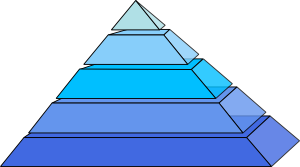
\includegraphics[width=1.1cm]{../Strukturfiler/FIGS/BluePyramid} & \begin{minipage}{\obsl}}{\end{minipage}\\ \end{tabular}\vspace{4mm}\newline}


% = Forudsætning = basis
\newenvironment{basis}{\begin{flushleft} \begin{itshape} }{\end{itshape} \end{flushleft}}


% = Opsummering =
\newenvironment{summary}{\clearpage\pagecolor{sumgul}\section{Opsummering}}{\newpage\pagecolor{white}}











% = Counter
\newcounter{opgavecount}[section]
\setcounter{opgavecount}{0}
\newcounter{spgcount}[opgavecount]
\setcounter{spgcount}{0}
\renewcommand{\thespgcount}{\alph{spgcount})}



% = EXERCISE = (DIVIDER)

\newcommand{\exercisebegin}[1][]{\bigskip\needspace{3\baselineskip}\refstepcounter{opgavecount}\titlegraphic{mingroen}\textcolor{mingroen}{\th{Opgave \theopgavecount \hspace*{1cm} #1}}\medskip\par}

% = QUIZEXERCISE = (DIVIDER)

\newcommand{\quizexercisebegin}[1][]{\bigskip\needspace{3\baselineskip}\refstepcounter{opgavecount}\titlegraphic{mingroen}\textcolor{mingroen}{\th{Quiz-Opgave \theopgavecount \hspace*{1cm} #1}}\medskip\par}

% = QUESTION =

\newenvironment{question}{\refstepcounter{spgcount}\begin{itemize}\item[\thespgcount]}{\end{itemize}\hspace*{\fill}}

% = VINK =

\newenvironment{vink}{\begin{tabular}{m{.9cm}<{\hspace*{2mm}}@{}|m{\obsl}@{}}\hspace*{-4pt}\raggedleft
\includegraphics[width=.9cm]{../Strukturfiler/FIGS/Think} & \begin{minipage}{\obsl}}{\end{minipage}\\ \end{tabular}\medskip\\}
	
% = FACIT =

\newenvironment{facit}{\begin{tabular}{m{.9cm}<{\hspace*{2mm}}@{}|m{\obsl}@{}}\hspace*{-4pt}\raggedleft
\includegraphics[width=.9cm]{../Strukturfiler/FIGS/Check} & \begin{minipage}{\obsl}}{\end{minipage}\\ \end{tabular}\medskip\\}








\newcommand{\afsnit}[1]{\bigskip\th{\titlegraphic{mingroen}\textcolor{mingroen}{#1}} \\ \rule[7pt]{.4\textwidth}{1pt} \vspace*{-2.5mm}\par}

% (DIVIDER):
\newcommand{\ugedagdatotitel}[4]{\pagebreak[4]\section{Semesteruge #1 -- #2 Dag \hspace*{1mm} (#3)} \vspace*{-4mm} \rule[5pt]{\textwidth}{1pt}\vspace*{-2.5mm} \begin{center}\large{\th{#4}}\end{center} \fancyhead[C]{\th{Semesteruge #1}}}

\newenvironment{skema}[1]{\definecolor{shadecolor}{rgb}{0.96,.98, 1.0} \setlength{\FrameSep}{6pt} \renewcommand{\FrameHeightAdjust}{10pt} \vspace*{-4pt}\begin{shaded} \begin{tabular}{#1}}{\end{tabular} \end{shaded} \vspace*{-7pt}}


% ========================

% MAKROER

%\newenvironment{matr}[1][]{\hspace*{-.8mm}\left[\hspace*{-1mm}\begin{array}{#1}}{\end{array}\hspace*{-1mm}\right]\hspace*{-.8mm}}
\newcommand{\bevisslut}{\begin{scriptsize} \begin{flushright} $ \blacksquare $ \end{flushright} \end{scriptsize}}

\newcommand{\tref}[2]{\hyperref[#1]{#2 \ref*{#1}}}
\newcommand{\thref}[2]{\hyperref[#1]{#2}}

\newcommand{\refA}[1]{\colorbox{yellow}{\ref{#1}}}
\newcommand{\hrefA}[2]{\colorbox{yellow}{\href{#1}{#2}}}
\newcommand{\trefA}[2]{\colorbox{yellow}{\hyperref[#1]{#2 \ref*{#1}}}}
\newcommand{\threfA}[2]{\colorbox{yellow}{\hyperref[#1]{#2}}}

\newenvironment{matr}[1]{\hspace*{-.8mm}\begin{bmatrix}\hspace*{-1mm}\begin{array}{#1}}{\end{array}\hspace*{-1mm}\end{bmatrix}\hspace*{-.8mm}}
\newcommand{\transp}{\hspace*{-.6mm}^{\top}}

\newcommand{\maengde}[2]{\left\lbrace \hspace*{-1mm} \begin{array}{c|c} #1 & #2 \end{array} \hspace*{-1mm} \right\rbrace}

\newenvironment{eqnalign}[1]{\setlength{\arraycolsep}{1.3pt}\begin{equation}\begin{array}{#1}}{\end{array}\end{equation}\par}
\newcommand{\eqnl}{\setlength{\arraycolsep}{1.3pt}}

\newcommand{\matind}[3]{{_\mathrm{#1}\mathbf{#2}_\mathrm{#3}}}
\newcommand{\vekind}[2]{{_\mathrm{#1}\mathbf{#2}}}
\newcommand{\jac}[2]{{\mathrm{Jacobi}_\mathbf{#1} (#2)}}
\newcommand{\diver}[2]{{\mathrm{div}\mathbf{#1} (#2)}}
\newcommand{\rot}[1]{{\mathbf{rot}\mathbf{(#1)}}}

\newcommand{\am}{\mathrm{am}}
\newcommand{\gm}{\mathrm{gm}}
\newcommand{\E}{\mathrm{E}}
\newcommand{\Span}{\mathrm{span}}
\newcommand{\mU}{\mathbf{U}}

\newcommand{\ms}{\medskip\\}
\newcommand{\bs}{\bigskip\\}

\newcommand{\mA}{\mathbf{A}}
\newcommand{\mB}{\mathbf{B}}
\newcommand{\mC}{\mathbf{C}}
\newcommand{\mD}{\mathbf{D}}
\newcommand{\mE}{\mathbf{E}}
\newcommand{\mF}{\mathbf{F}}
\newcommand{\mK}{\mathbf{K}}
\newcommand{\mI}{\mathbf{I}}
\newcommand{\mM}{\mathbf{M}}
\newcommand{\mN}{\mathbf{N}}
\newcommand{\mQ}{\mathbf{Q}}
\newcommand{\mT}{\mathbf{T}}
\newcommand{\mV}{\mathbf{V}}
\newcommand{\mW}{\mathbf{W}}
\newcommand{\mX}{\mathbf{X}}
\newcommand{\ma}{\mathbf{a}}
\newcommand{\mb}{\mathbf{b}}
\newcommand{\mc}{\mathbf{c}}
\newcommand{\md}{\mathbf{d}}
\newcommand{\me}{\mathbf{e}}
\newcommand{\mn}{\mathbf{n}}
\newcommand{\mr}{\mathbf{r}}
\newcommand{\mv}{\mathbf{v}}
\newcommand{\mw}{\mathbf{w}}
\newcommand{\mx}{\mathbf{x}}
\newcommand{\mxb}{\mathbf{x_{bet}}}
\newcommand{\my}{\mathbf{y}}
\newcommand{\mz}{\mathbf{z}}
\newcommand{\reel}{\mathbb{R}}
\newcommand{\mL}{\bm{\Lambda}} %Lambda-matrix
\newcommand{\mnul}{\bm{0}}
\newcommand{\trap}[1]{\mathrm{trap}(#1)}
\newcommand{\Det}{\operatorname{Det}}
\newcommand{\adj}{\operatorname{adj}}
\newcommand{\Ar}{\operatorname{Areal}}
\newcommand{\Vol}{\operatorname{Vol}}
\newcommand{\Rum}{\operatorname{Rum}}
\newcommand{\diag}{\operatorname{\bf{diag}}}
\newcommand{\bidiag}{\operatorname{\bf{bidiag}}}
\newcommand{\spanVec}[1]{\mathrm{span}\{#1\}}
\newcommand{\Div}{\operatorname{Div}}
\newcommand{\Rot}{\operatorname{\mathbf{Rot}}}

\newcommand{\Jac}{\operatorname{Jacobi}}
\newcommand{\Tan}{\operatorname{Tan}}
\newcommand{\Ort}{\operatorname{Ort}}
\newcommand{\Flux}{\operatorname{Flux}}
\newcommand{\Cmass}{\operatorname{Cm}}
\newcommand{\Imom}{\operatorname{Im}}
\newcommand{\Pmom}{\operatorname{Pm}}
\newcommand{\IS}{\operatorname{I}}
\newcommand{\IIS}{\operatorname{II}}
\newcommand{\IIIS}{\operatorname{III}}
\newcommand{\Le}{\operatorname{L}}
\newcommand{\app}{\operatorname{app}}
\newcommand{\M}{\operatorname{M}}
\newcommand{\re}{\mathrm{Re}}
\newcommand{\im}{\mathrm{Im}}

\newcommand{\compl}{\mathbb{C}} %de komplekse tal
\newcommand{\e}{\mathrm{e}} %eksponentialfunktionen. lodret 'e', og altså ikke kursiv ligesom andre bogstaver.





% Medialink: SCREEN: (QRcode) + thumbnail image + link på kodenummer (til qr.dtu.dk)
\newcommand{\onlinemedia}[3]{
	\begin{wrapfigure}{r}{3.2cm} 
		\vspace{-30pt} 
		\vspace{#1pt} 
		\begin{flushright} 
			\includegraphics[width=3cm]{qr/#2.png} 
			\tiny 
			\href{http://qr.dtu.dk/#2}{#2: #3}
			\normalsize  
		\end{flushright} 
		\vspace{-10pt} 
	\end{wrapfigure}
}
\newcommand{\onlinemediathumb}[3]{
	\begin{wrapfigure}{r}{3.2cm} 
		\vspace{-30pt} 
		\vspace{#1pt} 
		\begin{flushright} 
			\includegraphics[width=3cm]{qr/#2.png} 
			\includegraphics[width=3cm]{qr/#2_thumb.png} 
			\tiny 
			\href{http://qr.dtu.dk/#2}{#2: #3}
			\normalsize  
		\end{flushright} 
		\vspace{-10pt} 
	\end{wrapfigure}
}



% Index:
\usepackage{makeidx}
\makeindex
\newcommand\ind[2]{\index{#1}\textbf{\textit{\textcolor{black}{#2}}}}

% ###SERVER_EXCLUDE_BEGIN###
\externaldocument[NUID17-]{../../enoten/TN01-Talrum/Talrum}
\externaldocument[NUID1-]{../../enoten/TN02-Ligningssystemer/TNdriver}
\externaldocument[NUID2-]{../../enoten/TN03-Matricer_og_Matrixalgebra/Matricer_og_matrixalgebra}
\externaldocument[NUID3-]{../../enoten/TN04-Kvadratiske_matricer/TNdriver}
\externaldocument[NUID11-]{../../enoten/TN05-Determinanter/Determinanter}
\externaldocument[NUID12-]{../../enoten/TN06-GeometriskeVektorer/GeometriskeVektorer}
\externaldocument[NUID18-]{../../enoten/TN07-Vektorrum/VektorRum}
\externaldocument[NUID21-]{../../enoten/TN08-LinAfbildninger/LinAfbildninger}
\externaldocument[NUID23-]{../../enoten/TN09-Egenvaerdier_og_egenvektorer/TNdriver}
\externaldocument[NUID24-]{../../enoten/TN10-Diagonalisering_med_egenvektorer/TNdriver}
\externaldocument[NUID10-]{../../enoten/TN11-1.ordens_differentialligninger/TNdriver}
\externaldocument[NUID13-]{../../enoten/TN12-1.ordens_differentialligningssystemer/TNdriver}
\externaldocument[NUID14-]{../../enoten/TN13-2.ordens_differentialligninger/TNdriver}
\externaldocument[NUID27-]{../../enoten/TN14-Elemenataere_funktioner/Elementaere_Funktioner}
\externaldocument[NUID28-]{../../enoten/TN15-Funktioner2Variable/Funktioner_To_Variable}
\externaldocument[NUID29-]{../../enoten/TN16-Gradienter_og_Tangentplaner/Gradienter_og_Tangentplaner}
\externaldocument[NUID32-]{../../enoten/TN17-Taylor_formler/Taylor_Formler}
\externaldocument[NUID33-]{../../enoten/TN18-Taylor_2Var/Taylor_2Var}
\externaldocument[NUID34-]{../../enoten/TN19-SymMat/SymmetriskeMatricer}
\externaldocument[NUID35-]{../../enoten/TN20-KegleSnit/Keglesnit}
\externaldocument[NUID36-]{../../enoten/TN21-Riemann_Integral/Riemann_01}
\externaldocument[NUID37-]{../../enoten/TN22-Plan_Int/Plan_Int_01}
\externaldocument[NUID39-]{../../enoten/TN23-Flade_Int/Flade_Rum_Int_01}
\externaldocument[NUID40-]{../../enoten/TN24-Vektorfelter/Vektorfelter_01}
\externaldocument[NUID41-]{../../enoten/TN25-Flux/Flux_02}
\externaldocument[NUID42-]{../../enoten/TN26-Gauss/Gauss_01}
\externaldocument[NUID128-]{../../enoten/TN27-Stokes/Stokes_01}
\externaldocument[NUID43-]{../../enoten/TN29-KomplekseTal/KomplekseTal}

\externaldocument[NUID6-]{../../E-math-opgaver/Opgaver/opgU123}
\externaldocument[NUID19-]{../../E-math-opgaver/Opgaver/opgU45}
\externaldocument[NUID20-]{../../E-math-opgaver/Opgaver/opgU678}
\externaldocument[NUID25-]{../../E-math-opgaver/Opgaver/opgU910SD}
\externaldocument[NUID31-]{../../E-math-opgaver/OpgaverF11-U123/opgF123}
% \externaldocument[NUID9-]{../../E-math-opgaver/Opgaver/Dagsordner E10}
% ###SERVER_EXCLUDE_END###


% Begin document and set alternative chapter title:
\begin{document}
\renewcommand{\chaptername}{eNote}

\setcounter{chapter}{4} %SÆT DETTE TAL TIL 1 MINDRE END DET AKTUELLE TRANSFERNOTE-NUMMER!!

%%%%%%%%%%%%%%%%%%%%%%%%%%%%%%%%%%%%%%%%%%%%%
%%%%%%%%%%%%%%%%%%%%%%%%%%%%%%%%%%%%%%%%%%%%%
%%% HERFRA SKAL DU SKRIVE ELLER INDSÆTTE %%%%
%%% DEN FIL DU ØNSKER %%%%%%%%%%%%%%%%%%%%%%%
%%%%%%%%%%%%%%%%%%%%%%%%%%%%%%%%%%%%%%%%%%%%%
%%%%%%%%%%%%%%%%%%%%%%%%%%%%%%%%%%%%%%%%%%%%%

\chapter{Determinanter} \label{tn5}


\begin{basis}
I denne eNote ser vi på \ind{kvadratiske matricer}{kvadratiske matricer}; deres type er altså $n \times n$ for $n \geq 2$, se \tref{NUID3-tn4}{eNote}. Det er en fordel, men ikke absolut nødvendigt, at kende determinantbegrebet for $(2 \times 2)$-matricer på forhånd. Matrix-algebraen fra \tref{NUID2-tn3}{eNote} forudsættes bekendt (sum, produkt, transponering, invers, af matricer), samt den generelle løsningsmetode for lineære ligningssystemer fra \tref{NUID1-tn2}{eNote}.
\end{basis}

%%%%%%%%%%%%%%%%%%%%%%%%%%%%%%%%%%%%%%%%%%%%%%%%%%%%%%%%%%%%%
%%%%%%%%%%%%%%%%%%%%%%%%%%%%%%%%%%%%%%%%%%%%%%%%%%%%%%%%%%%%%
%%%%%%%%%%%%%%%%%%%%%%%%%%%%%%%%%%%%%%%%%%%%%%%%%%%%%%%%%%%%%

\ind{Determinant}{Determinanten} af en reel {\textit{kvadratisk}} $(n \times n)$-matrix $\mathbf{A}$ er et reelt tal, som vi betegner med \ind{$\det(\mathbf{A})$}{$\det(\mathbf{A})$} eller nogen gange kort med $|\mathbf{A}|$. Determinanten af en matrix kan betragtes som et mål for, hvor meget matricen 'vejer' - med fortegn; det vil vi illustrere visuelt og geometrisk for $(2 \times 2)$-matricer og for $(3 \times 3)$-matricer i \tref{NUID12-tn6}{eNote}. \\

Determinanten er en ganske bestemt {\textit{funktion}} af de i alt $n^{2}$ tal, der står som elementer i en $(n \times n)$-matrix.\\

For at definere -- og derefter beregne -- determinant-værdien af $(n \times n)$-matricer direkte ud fra de $n^{2}$ elementer i hver af matricerne har vi brug for to ting: Dels den velkendte determinant-formel for $(2 \times 2)$-matricer (se definition \ref{tn5.defDeterm22} nedenfor) og dels en  metode til at snitte en vilkårlig $(n \times n)$-matrix op i $(2 \times 2)$-matricer og derved definere og beregne vilkårlige determinanter ud fra determinanterne af disse $(2 \times 2)$-matricer.
%%%%%%%%%%%%%%%%%%%%%%%%%%%%%%%%%%%%%%%%%%%%%%%%%%%%%%%%%%%%%

\section{Determinanter af $(2 \times 2)-$matricer} \label{tn5.subsec22Matricer}

\begin{definition}[Determinanter af $(2 \times 2)-$matricer] \label{tn5.defDeterm22}
Lad $\mathbf{A}$ være den vilkårlige $(2 \times 2)-$matrix
\begin{equation} \label{tn5.22Matrix}
\mathbf{A} = \begin{matr}{cc}
             a_{11} & a_{12} \\
             a_{21} & a_{22} \\
\end{matr} \,  .
\end{equation}
Så er determinanten af $\mathbf{A}$ defineret ved:
\begin{equation} \label{tn5.eqDetFormel22}
\det(\mathbf{A}) = a_{11}\cdot a_{22} - a_{21}\cdot a_{12} \; .
\end{equation}
\end{definition}

\begin{exercise}[Invers $(2 \times 2)-$matrix]
Husk, at den inverse matrix $\mathbf{A}^{-1}$ til en regulær matrix $\mathbf{A}$ har den karakteristiske egenskab at $\mathbf{A}^{-1}\cdot \mathbf{A} = \mathbf{A}\cdot \mathbf{A}^{-1} = \mathbf{E}$.
Vis direkte ud fra (\ref{tn5.22Matrix}) og (\ref{tn5.eqDetFormel22}), at den inverse matrix $\mathbf{A}^{-1}$ til en $(2 \times 2)-$matrix $\mathbf{A}$ kan udtrykkes på følgende måde (når altså $\det(\mathbf{A}) \neq 0$) :
\begin{equation}
\mathbf{A}^{-1} = \frac{1}{\det(\mathbf{A})}\begin{matr}{rr}
                                        a_{22} & -a_{12} \\
                                        -a_{21} & a_{11} \\
                                    \end{matr} \,  .
\end{equation}
\end{exercise}

\begin{exercise}[Regneregler for $(2 \times 2)-$matricer]
For generelle kvadratiske matricer gælde en række fundamentale determinant-regneregler, som vil blive præsenteret i sætning \ref{tn5.thmDetEgenskaber} nedenfor.
Tjek allerede nu de tre første ligninger i  sætning \ref{tn5.thmDetEgenskaber} for $(2 \times 2)$-matricer $\mathbf{A}$ og $\mathbf{B}$. Brug direkte udregning af begge sider af ligningerne ved hjælp af (\ref{tn5.eqDetFormel22}).
\end{exercise}
%%%%%%%%%%%%%%%%%%%%%%%%%%%%%%%%%%%%%%%%%%%%%%%%%%%%%%%%%%%%%
\section{Snit-matricer}

\begin{definition}[Snitmatricer] \label{tn5.defSnitMat}
For en $(n \times n)$-matrix $\mathbf{A}$ defineres $(i,j)-$snitmatricen $\widehat{\mathbf{A}}_{ij}$ som den $((n-1) \times (n-1))$-undermatrix af $\mathbf{A}$, der fremkommer ved at slette hele række $i$ og hele søjle $j$ fra matricen $\mathbf{A}$.
\end{definition}

\begin{think}
Hver enkelt af de i alt $n^{2}$ snit-matricer $\widehat{\mathbf{A}}_{ij}$ (hvor $1\leq i \leq n$ og $1\leq j \leq n$)  er mindre end $\mathbf{A}$, de har typen $(n-1) \times (n-1)$ og derfor kun $(n-1)^{2}$ elementer.
\end{think}

\begin{example}[Snitmatricerne for en $(3 \times 3)-$matrix] \label{tn5.exampAmatrix33}
En $(3 \times 3)$-matrix $\mathbf{A}$ har i alt $9$ stk. $(2 \times 2)$-snitmatricer $\widehat{\mathbf{A}}_{ij}$. For eksempel, hvis
\begin{equation}
\mathbf{A} = \begin{matr}{rrr}
             0 & 2 & 1 \\
             1 & 3 & 2 \\
             0 & 5 & 1 \\
           \end{matr} \;,
\end{equation}
så er de $9$ snitmatricer hørende til $\mathbf{A}$ givet ved:
\begin{equation}
\begin{aligned}
\widehat{\mathbf{A}}_{11} &= \begin{matr}{rr}
                        3 & 2 \\
                        5 & 1 \\
                      \end{matr} \;, \quad
\widehat{\mathbf{A}}_{12} = \begin{matr}{rr}
                        1 & 2 \\
                        0 & 1 \\
                      \end{matr} \;, \quad
\widehat{\mathbf{A}}_{13} = \begin{matr}{rr}
                        1 & 3 \\
                        0 & 5 \\
                      \end{matr} \;,   \\
 \widehat{\mathbf{A}}_{21} &= \begin{matr}{rr}
                        2 & 1 \\
                        5 & 1 \\
                      \end{matr} \;, \quad
\widehat{\mathbf{A}}_{22} = \begin{matr}{rr}
                        0 & 1 \\
                        0 & 1 \\
                      \end{matr} \;, \quad
\widehat{\mathbf{A}}_{23} = \begin{matr}{rr}
                        0 & 2 \\
                        0 & 5 \\
                      \end{matr} \;,    \\
 \widehat{\mathbf{A}}_{31} &= \begin{matr}{rr}
                        2 & 1 \\
                        3 & 2 \\
                      \end{matr} \;, \quad
\widehat{\mathbf{A}}_{32} = \begin{matr}{rr}
                        0 & 1 \\
                        1 & 2 \\
                      \end{matr} \;, \quad
\widehat{\mathbf{A}}_{33} = \begin{matr}{rr}
                        0 & 2 \\
                        1 & 3 \\
                      \end{matr} \;.
\end{aligned}
\end{equation}
Deres respektive determinanter er determinanter af $(2 \times 2)-$matricer, og kan hver for sig direkte beregnes ud fra definitionen \ref{tn5.defDeterm22} ovenfor:
\begin{eqnalign}{rclrclrcl}
\det(\widehat{\mathbf{A}}_{11}) & = & -7  \;, \; &
\det(\widehat{\mathbf{A}}_{12}) & = & 1  \;, \; &
\det(\widehat{\mathbf{A}}_{13}) & = & 5  \; ,    \\
\det(\widehat{\mathbf{A}}_{21}) & = & -3  \;, \; &
\det(\widehat{\mathbf{A}}_{22}) & = & 0  \;, \; &
\det(\widehat{\mathbf{A}}_{23}) & = & 0  \;,   \\
\det(\widehat{\mathbf{A}}_{31}) & = & 1  \;, \; &
\det(\widehat{\mathbf{A}}_{32}) & = & -1  \;,\; &
\det(\widehat{\mathbf{A}}_{33}) & = & -2  \; .
\end{eqnalign}

\end{example}

%%%%%%%%%%%%%%%%%%%%%%%%%%%%%%%%%%%%%%%%%%%%%%%%%%%%%%%%%%%%%
%%%%%%%%%%%%%%%%%%%%%%%%%%%%%%%%%%%%%%%%%%%%%%%%%%%%%%%%%%%%%
%%%%%%%%%%%%%%%%%%%%%%%%%%%%%%%%%%%%%%%%%%%%%%%%%%%%%%%%%%%%%

\section{Induktiv definition af determinanter} \label{afsnit.inddefdet}

Determinanten af en $3 \times 3$ matrix kan nu defineres ud fra determinanterne af $3$ af sine $9$ snitmatricer, og generelt: Determinanten af en $n \times n$ matrix defineres ved hjælp af determinanterne af de $n$ snitmatricer der hører til en (frit valgt men fast) række $r$
på følgende måde, som naturligt nok kaldes \ind{opløsning efter $r$-te række}{opløsning efter $r$-te række}:

\begin{definition}[Determinanter defineres ved opløsning]\label{tn5.defDeterminantRaekke}
For en vilkårlig værdi af rækkeindeks $r$ defineres determinanten af
en given $(n \times n)$-matrix $\mathbf{A}$ induktivt på følgende måde:
\begin{equation} \label{tn5.eqDeterminant}
\det(\mathbf{A}) = \sum_{j=1}^{n}(-1)^{r+j}a_{rj}\det(\widehat{\mathbf{A}}_{rj})\quad .
\end{equation}
\end{definition}

\begin{info}
Vi benytter her og senere følgende korte skrivemåder og notationer for summer og produkter
af mange led, f.eks. $n$ givne reelle tal $c_{1}, c_{2}, \ldots, c_{n-1}, c_{n}$:
\begin{equation}
\begin{aligned}
c_{1}+ c_{2} + \cdots + c_{n-1} + c_{n} &= \sum_{i=1}^{n} c_{i} \; , \quad \textrm{og}\\
c_{1} \cdot c_{2} \cdot \cdots \cdot c_{n-1} \cdot c_{n} &= \prod_{i=1}^{n} c_{i} \quad .
\end{aligned}
\end{equation}
\end{info}

\begin{example} [Opløsning af en determinant efter 1. række]\label{tn5.detAf3x3matrix}
Vi vil benytte definition \ref{tn5.defDeterminantRaekke} direkte til at beregne determinanten af den matrix $\mathbf{A}$ som er givet i eksempel \ref{tn5.exampAmatrix33}. Vi vælger $r=1$ og har så brug for de tre snitmatrix-determinanter, $\det(\widehat{\mathbf{A}}_{11}) = -7$, $\det(\widehat{\mathbf{A}}_{12}) = 1$, og $\det(\widehat{\mathbf{A}}_{13})= 5$, som vi allerede har udregnet ovenfor i eksempel \ref{tn5.exampAmatrix33}:
\begin{equation}
\begin{aligned}
\det(\mathbf{A}) &=  \sum_{j=1}^{n}(-1)^{1+j}a_{1j}\det(\widehat{\mathbf{A}}_{1j}) \\
&= (-1)^{1+1}\cdot 0 \cdot\det(\widehat{\mathbf{A}}_{11}) + (-1)^{1+2}\cdot2\cdot\det(\widehat{\mathbf{A}}_{12}) +
(-1)^{1+3} \cdot 1 \cdot \det(\widehat{\mathbf{A}}_{13}) \\
&= 0 - 2 + 5 = 3 \quad .
\end{aligned}
\end{equation}
\end{example}

\begin{obs}
Læg mærke til, at snitmatricernes determinanter skal ganges med det element i $\mathbf{A}$ som står på plads $(r,j)$ og med fortegns-faktoren $(-1)^{r+j}$ før de lægges sammen. Og læg mærke til, at snitmatricernes determinanter jo selv kan 'trævles op' til en bestemmelse af determinanter af endnu mindre matricer, således at vi til sidst ender med 'kun' at skulle bestemme vægtede summer af determinanter af $(2 \times 2)-$matricer!
\end{obs}


\begin{exercise} [Valg af 'opløsningsrække' er ligegyldig]\label{tn5.exercAlterOpl}
Vis direkte ved beregning, at vi får samme værdi for determinanten ved at bruge en af de andre to rækker til opløsningen af determinanten i eksempel \ref{tn5.exampAmatrix33}.
\end{exercise}

\begin{definition}[Alternativ: Opløsning efter søjle] \label{tn5.defDeterminantSoejle}
Determinanten af en given $(n \times n)-$matrix $\mathbf{A}$ kan alternativt defineres induktivt ved
opløsning efter en vilkårlig valgt \textit{søjle} :
\begin{equation} \label{tn5.eqDeterminantSoejle}
\det(\mathbf{A}) = \sum_{i=1}^{n}(-1)^{i+s}a_{i\,s}\det(\widehat{\mathbf{A}}_{i\,s}) \quad .
\end{equation}
Her er opløsningen udtrykt ved opløsning efter søjle $s$.
\end{definition}

Som det er antydet allerede med definitionerne og som vist i det konkrete tilfælde med matricen i eksempel \ref{tn5.exampAmatrix33}, er det ligegyldigt, hvilken række (eller søjle) man opløser efter:

\begin{theorem}[Valg af opløsnings-række eller -søjle er ligegyldig]
De to definitioner, \ref{tn5.defDeterminantRaekke} og \ref{tn5.defDeterminantSoejle}, af determinanten af en kvadratisk matrix giver samme værdi og er uafhængige af valg af række hhv. søjle til de respektive opløsninger.
\end{theorem}

\begin{exercise}[Valg af 'opløsningssøjle' er ligegyldig]
Vis direkte ved beregning, at vi får samme værdi for determinanten i \ref{tn5.exampAmatrix33} ved at bruge søjle-opløsning efter en vilkårlig af de tre søjler i $\mathbf{A}$.
\end{exercise}

\begin{think}
Det er selvsagt smartest at opløse efter en række, eller en søjle, som indeholder en masse $0$'er.
\end{think}

\begin{exercise}[Determinanter af nogle større matricer]
Benyt de ovenfor givne anvisninger og resultater til at finde determinanten af hver af følgende matricer:
\begin{equation}
\begin{matr}{cccc}
    0 & 2 & 7 & 1 \\
    1 & 3 & 0 & 2 \\
    0 & 0 & 1 & 0 \\
    0 & 5 & 8 & 1 \\
  \end{matr} \;, \;\begin{matr}{ccccc}
                                0 & 2 & 1 & 0 & 5 \\
                                1 & 3 & 2 & 0 & 2 \\
                                0 & 5 & 1 & 0 & 1 \\
                                0 & 0 & 1 & 0 & 0 \\
                                5 & 2 & 7 & 1 & 9 \\
                              \end{matr} \;, \; \begin{matr}{cccccc}
                                                      0 & 0 & 2 & 1 & 5 & 3 \\
                                                      0 & 1 & 3 & 2 & 2 & 1 \\
                                                      0 & 0 & 5 & 1 & 1 & 4 \\
                                                      1 & 0 & 0 & 0 & 0 & 0 \\
                                                      0 & 0 & 1 & 0 & 0 & 0 \\
                                                      0 & 5 & 2 & 7 & 1 & 9 \\
                                                    \end{matr} \;.
\end{equation}
\end{exercise}

\begin{aha}
Hvis der er mange $0$'er i en matrix, så er det meget lettere at beregne dens determinant! Specielt hvis alle elementer i en række (henholdsvis søjle) er $0$ pånær \'{e}t element, så er det klart smartest at opløse efter den række (henholdsvis søjle).
Og det er tilladt at 'skaffe' sig en masse $0$'er ved de velkendte rækkeoperationer, hvis man blot holder øje med, hvilke konstanter der divideres med og hvor mange gange der byttes om på rækkerne. Se sætning \ref{tn5.thmEgenskaberDeterm} og eksempel \ref{tn5.exampTrappeDet} nedenfor.
\end{aha}

%%%%%%%%%%%%%%%%%%%%%%%%%%%%%%%%%%%%%%%%%%%%%%%%%%%%%%%%%%%%%
%%%%%%%%%%%%%%%%%%%%%%%%%%%%%%%%%%%%%%%%%%%%%%%%%%%%%%%%%%%%%
%%%%%%%%%%%%%%%%%%%%%%%%%%%%%%%%%%%%%%%%%%%%%%%%%%%%%%%%%%%%%

\section{Beregningstekniske egenskaber ved determinanter}


Vi samler her nogle af de vigtigste redskaber, som ofte benyttes til beregning og inspektion af determinanter af matricer.\\

Det er ikke svært at vise følgende sætning, f.eks. direkte ved først at opløse efter første søjle eller efter første række, hvorefter mønsteret viser sig:

\begin{theorem}[Matricer med $0$ over eller under diagonalen] \label{tn5.thmTriangMatrixDet}
Hvis en $(n \times n)-$matrix har lutter $0$'er over eller under diagonalen, så er determinanten givet ved produktet af diagonalelementerne.
\end{theorem}

Specielt har vi derfor:

\begin{theorem}[Determinanten af en diagonalmatrix]
Lad $\mL$ betegne en $(n \times n)$-\ind{diagonalmatrix}{diagonalmatrix} med diagonal-elementerne $\lambda_{1}, \lambda_{2}, ..., \lambda_{n}$ og ellers med $0$'er udenfor diagonalen:
\begin{equation}
 \bm{\Lambda} = \diag(\lambda_{1}, \lambda_{2}, \cdots, \lambda_{n}) =
\begin{bmatrix}
\lambda_{1} & 0 & \cdots & 0 \\
0 & \lambda_{2} & \cdots & 0 \\
\vdots & \vdots & \ddots & \vdots \\
0 & 0 & \ldots & \lambda_{n}
\end{bmatrix} \; .
\end{equation}
Så er determinanten
\begin{equation}
\det(\mL) = \lambda_{1}\,\lambda_{2} \cdot \cdot \cdot \lambda_{n}  = \prod_{i=1}^{n} \lambda_{i}
\end{equation}
\end{theorem}

\begin{exercise}[Determinanten af en bi-diagonalmatrix]
Bestem determinanten af $(n \times n)-$ \ind{bi-diagonal-matrix}{bi-diagonal-matricen} med vilkårligt givne værdier $\mu_{1}$, . . . , $\mu_{n}$ i bidiagonalen og $0$'er udenfor:
\begin{equation}
\mathbf{M} = \bidiag(\mu_{1}, \mu_{2}, \cdots, \mu_{n}) =
\begin{matr}{cccc}
0 &  \cdots & 0 &\mu_{1} \\
0  & \cdots & \mu_{2} & 0 \\
\vdots & \reflectbox{$\ddots$} & \vdots & \vdots \\
\mu_{n} & \ldots & 0 & 0
\end{matr} \; .
\end{equation}
\end{exercise}

For generelle matricer og derfor også for kvadratiske matricer gælder som bekendt fra \tref{NUID1-tn2}{eNote}, at de kan omformes til trappeform ved brug af rækkeoperationer.
Hvis man holder godt øje med, hvad der sker ved hvert skridt i den omformning,
så kan determinanten af matricen direkte aflæses ud fra processen. Determinanten af en matrix opfører sig nemlig 'pænt' selvom der udføres rækkeoperationer på matricen:


\begin{theorem} [Rækkeoperationers indflydelse på determinanten]\label{tn5.thmEgenskaberDeterm}
Determinanten har følgende egenskaber:
\begin{enumerate}
\item Hvis alle elementer i en række i $\mathbf{A}$ er $0$, så er determinanten $0$, $\det(\mathbf{A}) = 0$.
\item Hvis to rækker ombyttes i $\mathbf{A}$, $R_{i} \leftrightarrow R_{j}$,  så skifter determinanten fortegn.
\item Hvis alle elementerne i en række i $\mathbf{A}$ ganges med en konstant $k$, $k \cdot R_{i}$,  så bliver determinanten ganget med $k$.
\item Hvis to rækker i en matrix $\mathbf{A}$ er ens, så er $\det(\mathbf{A}) = 0$.
\item En rækkeoperation af typen $R_{j} + k \cdot R_{i}$ hvor $i \neq j$ ændrer ikke determinanten.
\end{enumerate}
\end{theorem}


Som antydet ovenfor følger det af disse egenskaber ved determinantfunktionen, at den velkendte reduktion af en given matrix $\mathbf{A}$ til trappeform, $\trap{\mathbf{A}}$, via rækkeoperationer som beskrevet i \tref{NUID1-tn2}{eNote}, faktisk {\textit{indeholder}} en helt eksplicit beregning af determinanten af $\mathbf{A}$. Vi illustrerer med et simpelt eksempel:

\begin{example}[Inspektion af determinant ved reduktion til trappeform] \label{tn5.exampTrappeDet}
Vi betragter $(3 \times 3)-$matricen $\mathbf{A}_{1} = \mathbf{A}$ fra eksempel \ref{tn5.exampAmatrix33}:
\begin{equation}
\mathbf{A}_{1} =  \begin{matr}{rrr}
             0 & 2 & 1 \\
             1 & 3 & 2 \\
             0 & 5 & 1 \\
           \end{matr}
\end{equation}
Vi reducererden  til trappeform på sædvanlig måde med Gauss--Jordan rækkeoperationer og holder hele tiden øje med, hvad der sker med determinanten
ved at bruge reglerne fra \ref{tn5.thmEgenskaberDeterm} (og ved eventuelt derudover at checke dem med direkte udregninger):

Operation: Ombyt række $1$ og række $2$, $R_{1} \leftrightarrow R_{2}$ : Determinanten skifter fortegn :
\begin{equation}
\det(\mathbf{A}_{2}) = -\det(\mathbf{A}_{1}) \;:
\end{equation}
\begin{equation}
\mathbf{A}_{2} =  \begin{matr}{rrr}
             1 & 3 & 2 \\
             0 & 2 & 1 \\
             0 & 5 & 1 \\
           \end{matr}
\end{equation}
Operation: $\tiny{\frac{1}{2}}R_{2}$, række 2 ganges med $\tiny{\frac{1}{2}}$  : Determinanten ganges med $\tiny{\frac{1}{2}}$ :
\begin{equation}
\det(\mathbf{A}_{3}) = \frac{1}{2}\det(\mathbf{A}_{2}) = -\frac{1}{2}\det(\mathbf{A}_{1}) \;:
\end{equation}
\begin{equation}
\mathbf{A}_{3} =  \begin{matr}{ccc}
             1 & 3 & 2 \\
             0 & 1 & 1/2 \\
             0 & 5 & 1 \\
           \end{matr}
\end{equation}
Operation: $R_{1}- 3R_{2}$: Determinanten uændret:
\begin{equation}
\det(\mathbf{A}_{4}) =   \det(\mathbf{A}_{3}) = \frac{1}{2}\det(\mathbf{A}_{2}) = -\frac{1}{2}\det(\mathbf{A}_{1}) \; :
\end{equation}
\begin{equation}
\mathbf{A}_{4} =  \begin{matr}{ccc}
             1 & 0 & 1/2 \\
             0 & 1 & 1/2 \\
             0 & 5 & 1 \\
           \end{matr}
\end{equation}
Operation: $R_{3}- 5R_{2}$: Determinanten uændret:
    \begin{equation}
    \det(\mathbf{A}_{5}) =  \det(\mathbf{A}_{4}) =   \det(\mathbf{A}_{3}) = \frac{1}{2}\det(\mathbf{A}_{2}) = -\frac{1}{2}\det(\mathbf{A}_{1}) \;:
    \end{equation}
\begin{equation}
\mathbf{A}_{5} =  \begin{matr}{rrr}
             1 & 0 & 1/2 \\
             0 & 1 & 1/2 \\
             0 & 0 & -3/2 \\
           \end{matr}
\end{equation}
Determinanten er nu diagonal-produktet fordi alle elementerne under diagonalen er $0$, se sætning \ref{tn5.thmTriangMatrixDet}. Ialt har vi derfor:
\begin{equation}
-\frac{3}{2} =    \det(\mathbf{A}_{5}) =  \det(\mathbf{A}_{4}) =   \det(\mathbf{A}_{3}) = \frac{1}{2}\det(\mathbf{A}_{2}) = -\frac{1}{2}\det(\mathbf{A}_{1}) \;:
\end{equation}
Heraf direkte -- ved at læse 'baglæns':
\begin{equation}
-\frac{1}{2}\det(\mathbf{A}_{1}) = -\frac{3}{2} \;,
\end{equation}
således at
\begin{equation}
\det(\mathbf{A}_{1}) = 3 \;.
\end{equation}
\end{example}

Derudover har vi følgende sammenhæng mellem rang og determinant; determinanten afslører simpelthen, om matricen er singulær eller regulær:

\begin{theorem}[Rang versus determinant]
Rangen af en kvadratformet $(n \times n)$-matrix $\mathbf{A}$ er skarpt mindre end $n$ hvis og kun hvis determinanten af $\mathbf{A}$ er $0$. Med andre ord, $\mathbf{A}$ er singulær hvis og kun hvis $\det(\mathbf{A}) = 0$.
\end{theorem}

Hvis en matrix indeholder en variabel, en parameter, så er determinanten af matricen en funktion af denne
parameter; i anvendelserne af matrix-algebra er det ofte ret afgørende at kunne finde nulpunkterne for den
funktion -- netop fordi den tilhørende matrix er singulær for de værdier af parameteren, så der måske ikke findes en (entydig) løsning til
det tilsvarende lineære ligningssystem der har matricen som koefficientmatrix.

\begin{exercise}[Determinant af matrix med variabel] \label{tn5.exercReduktionDet}
Givet matricen
\begin{equation}
\mathbf{A} = \begin{matr}{cccc}
1 & a & a^{2} & a^{3} \\
1 & 0 & a^{2} & a^{3} \\
1 & a & a & a^{3} \\
1 & a & a^{2} & a
\end{matr} \, , \; \textrm{hvor $a \in \Bbb R$.}
\end{equation}
\begin{enumerate}
\item Bestem determinanten af ${\bf{A}}$ som et polynomium i $a$.
\item Bestem rødderne i dette polynomium.
\item Find rangen af ${\mathbf{A}}$ for $a \, \in \,
\{-4, -3, -2, -1, 0, 1, 2, 3, 4\}$ . Hvad har rangen med de fundne
rødder i determinanten at gøre?
\item Find rangen af ${\mathbf{A}}$ for alle $a$.
\end{enumerate}
\end{exercise}

\begin{theorem}[Regneregler for determinanter] \label{tn5.thmDetEgenskaber}
Lad $\mathbf{A}$ og $\mathbf{B}$ betegne to $(n \times n)-$matricer. Så gælder:
\begin{enumerate}
\item $ \det(\mathbf{A}) = \det(\mathbf{A}\transp) $
\item $ \det(\mathbf{A}\mathbf{B}) = \det(\mathbf{A})\det(\mathbf{B}) $
\item $ \det(\mathbf{A}^{-1}) = \left(\det(\mathbf{A})\right)^{-1} $, når blot $\mathbf{A}$ er regulær, altså $\det(\mathbf{A}) \neq 0$
\item $ \det(\mathbf{A}^{k}) = (\det(\mathbf{A}))^{k} $, for alle $k \geq 1$.
\item $ \det(\mathbf{B}^{-1}\mathbf{A}\mathbf{B}) = \det(\mathbf{A}) $, når blot $\mathbf{B}$ er regulær, det vil sige $\det(\mathbf{B}) \neq 0$.
\end{enumerate}
\end{theorem}

\begin{exercise}
Bevis de $3$ sidste ligninger i sætning \ref{tn5.thmDetEgenskaber} ved at bruge ligningen $\det(\mathbf{A}\mathbf{B}) = \det(\mathbf{A})\det(\mathbf{B})$.
\end{exercise}

\begin{exercise}[Determinanten af en sum er ikke determinantsummen]
Vis med et simplest muligt eksempel, at determinant-funktionen $\det( )$ {\textit{ikke}} er additiv, altså find to $(n \times n)-$matricer $\mathbf{A}$ og $\mathbf{B}$
således at
\begin{equation}
\det(\mathbf{A} + \mathbf{B}) \neq \det(\mathbf{A}) + \det(\mathbf{B}) \;.
\end{equation}
\end{exercise}


\begin{exercise} [Brug af regnereglerne for determinanter] \label{tn5.exercLA39}
Lad $a$ betegne et reelt tal. Der er  givet følgende matricer:
\begin{equation}
\mathbf{A} = \begin{matr}{rrr}
             3 & 4 & 4 \\
             1 & a & 2 \\
             2 & 3 & 3 \\
           \end{matr} \; \textrm{og} \; \mathbf{B} = \begin{matr}{rrr}
                                                   2 & -1 & 0 \\
                                                   -5 & 3 & -1 \\
                                                   0 & 1 & a \\
                                                 \end{matr} \,.
\end{equation}
\begin{enumerate}
\item Find $\det(\mathbf{A})$ og $\det(\mathbf{B})$.
\item Find $\det(\mathbf{A\,B})$ og $\det\left(\left(\mathbf{A}\transp \mathbf{B}\right)^{4}\right)$.
\item Angiv de værdier af $a$, for hvilke $\mathbf{A}$ er regulær og find for disse værdier af $a$ udtrykket for
$\det(\mathbf{A}^{-1})$.
\end{enumerate}
\end{exercise}

%%%%%%%%%%%%%%%%%%%%%%%%%%%%%%%%%%%%%%%%%%%%%%%%%%%%%%%%%%%%%
%%%%%%%%%%%%%%%%%%%%%%%%%%%%%%%%%%%%%%%%%%%%%%%%%%%%%%%%%%%%%
%%%%%%%%%%%%%%%%%%%%%%%%%%%%%%%%%%%%%%%%%%%%%%%%%%%%%%%%%%%%%

\section{Advanced: Det karakteristiske polynomium} \label{tn5.secKarakterPol}

Materialet i dette afsnit hører beregningsteknisk naturligt hjemme i denne eNote om determinanter, men det er først senere -- ved
løsning af de såkaldte egenværdiproblemer, at vi virkelig får brug for de karakteristiske polynomier.\\

For en given kvadratformet matrix $\mathbf{A}$ defineres den tilhørende \ind{karakteristisk matrix}{karakteristiske matrix}
og det tilhørende \ind{karakteristiske polynomium}{karakteristisk polynomium} på følgende måde:

\begin{definition}[Den karakteristiske matrix]
Lad $\mathbf{A}$ være en $(n \times n)-$matrix. Den tilhørende {\textit{karakteristiske matrix}} er følgende matrix-funktion af den reelle variable $\lambda$:
\begin{equation}
\mathbf{K}_{\mathbf{A}}(\lambda) = \mathbf{A} - \lambda\,\mathbf{E} \;, \;\textrm{hvor} \;\lambda \in \mathbb{R} \;,
\end{equation}
hvor $\mathbf{E} = \mathbf{E}_{n \times n} = \diag(1, 1, . . . , 1)$ er $(n \times n)-$enhedsmatricen.

\end{definition}

\begin{example} [En karakteristisk matrix] \label{exampKarakMat}
Givet en $(3 \times 3)-$matrix $\mathbf{A}$ ved
\begin{equation}
\mathbf{A} = \begin{matr}{rrr}
             3 & -2 & 0 \\
             0 & 1 & 0 \\
             1 & -1 & 2 \\
           \end{matr} \;.
\end{equation}
Så er
\begin{equation}
\mathbf{K}_{\mathbf{A}}(\lambda) = \mathbf{A} - \lambda\,\mathbf{E} = \begin{matr}{ccc}
            3 -\lambda & -2 & 0 \\
             0 & 1-\lambda  & 0 \\
             1 & -1 & 2-\lambda  \\
           \end{matr} \;.
\end{equation}
\end{example}


Det tilhørende \ind{karakteristiske polynomium}{karakteristiske polynomium} for matricen $\mathbf{A}$ er dernæst følgende reelle polynomium af variablen $\lambda$:

\begin{definition}[Det karakteristiske polynomium] \label{tn5.defKarakPol}
Givet den kvadratiske matrix $\mathbf{A}$, så defineres det karakteristiske polynomium for $\mathbf{A}$ således:
\begin{equation}
\mathcal{K}_{\mathbf{A}}(\lambda) = \det(\mathbf{K}_{\mathbf{A}}(\lambda)) = \det(\mathbf{A} - \lambda\,\mathbf{E}) \;, \;\textrm{hvor} \;\lambda \in \mathbb{R} \;.
\end{equation}
\end{definition}





\begin{example}[Et karakteristisk polynomium]
Med  $\mathbf{A}$ som i eksempel \ref{exampKarakMat} får vi følgende karakteristiske polynomium for $\mathbf{A}$ ved at opløse den karakteristiske matrix efter sidste søjle:
\begin{equation}
\begin{aligned}
\mathcal{K}_{\mathbf{A}}(\lambda) &= \det\left(\begin{matr}{ccc}
            3 -\lambda & -2 & 0 \\
             0 & 1-\lambda  & 0 \\
             1 & -1 & 2-\lambda  \\
           \end{matr}\right) \\
&= (-1)^{3+3}(2-\lambda) \det \left(\begin{matr}{cc}
                     3 - \lambda & -2 \\
                     0 & 1-\lambda \\
                   \end{matr}
\right) \\
&= (2-\lambda)(3 - \lambda)(1-\lambda) \;.
\end{aligned}
\end{equation}
Det karakteristiske polynomium for  $\mathbf{A}$ har altså rødderne $1$, $2$, og $3$.
\end{example}

\begin{info}
%Det karakteristiske polynomium $\mathcal{K}_{\mathbf{A}}(\lambda)$ -- og især de $\lambda$-værdier for hvilke  $\mathcal{K}_{\mathbf{A}}(\lambda) = 0$, altså rødderne i polynomiet -- spiller en afgørende rolle for forståelsen af og anvendelsen af $\mathbf{A}$-matricens operative egenskaber, som vil blive beskrevet udførligt i eNote REFERENCE \ref{TN}. Rødderne i det karakteristiske polynomium for en matrix kaldes matricens egen-værdier. Det forekommer ofte, at nogle af (måske endda alle) rødderne er komplekse. Hvis matricen er symmetrisk (dvs. $\mathbf{A} = \mathbf{A}\transp$)\, , så  er alle egenværdierne dog reelle, se eNote REFERENCE \ref{TN}.
Det karakteristiske polynomium $\mathcal{K}_{\mathbf{A}}(\lambda)$ -- og især de $\lambda$-værdier for hvilke $\mathcal{K}_{\mathbf{A}}(\lambda) = 0$, altså rødderne i polynomiet -- spiller en afgørende rolle for forståelsen af og anvendelsen af $\mathbf{A}$-matricens operative egenskaber, som vil blive beskrevet i eNoten om egenværdier og egenvektorer. Rødderne i det karakteristiske polynomium for en matrix kaldes matricens egenværdier.
\end{info}

\begin{exercise}[Graden af det karakteristiske polynomium]
Argument\'{e}r for, at det karakteristiske polynomium $\mathcal{K}_{\mathbf{A}}(\lambda)$ for en $(n \times n)-$matrix $\mathbf{A}$ er et polynomium i $\lambda$ af graden $n$.
\end{exercise}

\begin{exercise}[Nogle karakteristiske polynomier og deres rødder]
Bestem de karakteristiske polynomier for følgende matricer og find alle reelle rødder i hvert af polynomierne:
\begin{equation}
\mathbf{A}_{1} = \begin{matr}{cc}
                 1 & 2 \\
                 3 & 4 \\
               \end{matr} \;, \;\mathbf{A}_{2} = \diag(a_{1}, a_{2}, a_{3})\;, \;\mathbf{A}_{3} = \bidiag(b_{1}, b_{2}, b_{3}) \; .
\end{equation}
\end{exercise}

\begin{exercise}[Find matricer med givne karakter-egenskaber]
Konstruér to $(4 \times 4)$-matricer $\mathbf{A}$ og $\mathbf{B}$  sådan, at den ene har lutter reelle rødder i sit karakteristiske polynomium, og sådan at den anden ikke har nogen som helst reelle rødder i sit karakteristiske polynomium.
\end{exercise}


%%%%%%%%%%%%%%%%%%%%%%%%%%%%%%%%%%%%%%%%%%%%%%%%%%%%%%%%%%%%%
%%%%%%%%%%%%%%%%%%%%%%%%%%%%%%%%%%%%%%%%%%%%%%%%%%%%%%%%%%%%%
%%%%%%%%%%%%%%%%%%%%%%%%%%%%%%%%%%%%%%%%%%%%%%%%%%%%%%%%%%%%%



\section{Advanced: Cramer's løsningsmetode} \label{tn5.secCramer}

Hvis $\mathbf{A}$ er en regulær $n \times n$ matrix og $\mathbf{b} = (b_{1}, . . . , b_{n})$ er en vilkårlig vektor i $\mathbb{R}^{n}$, så findes der (som det også er bekendt fra \tref{NUID1-tn2}{eNote} (regulær koefficientmatrix)) præcis én løsning $\mathbf{x} = (x_{1}, . . . , x_{n}) $ til det lineære ligningssystem $\mathbf{A}\mathbf{x} = \mathbf{b}$ og vi har i den eNote fundet metoder til at finde løsningen.

Cramer's metode til løsning af sådanne ligningssystemer er en \textit{direkte} metode. Den består essentielt i at udregne passende determinanter af matricer, der konstrueres ud fra $\mathbf{A}$ og $\mathbf{b}$ og så skrive løsningen ned direkte ud fra de beregnede determinanter.

\begin{theorem} [Cramer's løsningsformel]\label{tn5.thmCramer}
Lad $\mathbf{A}$ være en regulær $n \times n$ matrix og lad $\mathbf{b} = (b_{1}, . . . , b_{n})$ betegne en vilkårlig vektor i $\mathbb{R}^{n}$. Så findes der (som det også er bekendt fra \tref{NUID1-tn2}{eNote} (regulær koefficientmatrix)) præcis én løsning $\mathbf{x} = (x_{1}, . . . , x_{n}) $ til det lineære ligningssystem
\begin{equation} \label{tn5.eqCramerSys}
\mathbf{A}\mathbf{x} = \mathbf{b} \;,
\end{equation}
og elementerne i den løsning er givet ved:
\begin{equation} \label{tn5.eqCramerSol}
x_{j} = \frac{1}{\det(\mathbf{A})}\det(\mathbf{A}\dag_{\small{j}}^{\mathbf{b}}) \;,
\end{equation}
hvor $\mathbf{A}\dag_{\small{j}}^{\mathbf{b}}$ betegner den $(n \times n)-$matrix, der fremkommer ved at erstatte søjle $j$ i $\mathbf{A}$ med $\mathbf{b}$.
\end{theorem}

\begin{explain}[Hvad $\dag$ betyder]
Hvis $\mathbf{A}$ er følgende matrix (fra eksempel \ref{tn5.exampAmatrix33})
\begin{equation}
\mathbf{A} = \begin{matr}{rrr}
             0 & 2 & 1 \\
             1 & 3 & 2 \\
             0 & 5 & 1 \\
           \end{matr} \;,
\end{equation}
og hvis vi lader $\mathbf{b} = (b_{1}, b_{2}, b_{3})$, så er
\begin{equation} \label{tn5.eqDagger}
\mathbf{A}\dag_{\small{1}}^{\mathbf{b}} = \begin{matr}{rrr}
                                     b_{1} & 2 & 1 \\
                                     b_{2} & 3 & 2 \\
                                     b_{3} & 5 & 1 \\
                                   \end{matr} \,\, , \,\,
                                 \mathbf{A}\dag_{\small{2}}^{\mathbf{b}} = \begin{matr}{rrr}
                                     0 & b_{1} & 1 \\
                                     1 & b_{2} & 2 \\
                                     0 & b_{3} & 1 \\
                                   \end{matr} \,\, , \,\,
                                 \mathbf{A}\dag_{\small{3}}^{\mathbf{b}} = \begin{matr}{rrr}
                                     0 & 2 & b_{1} \\
                                     1 & 3 & b_{2} \\
                                     0 & 5 & b_{3} \\
                                   \end{matr} \,\, .
\end{equation}
\end{explain}

\begin{exercise}[Brug af Cramer's løsningsformel]
Hvis vi specielt lader $\mathbf{A}$ være den samme matrix som ovenfor og nu helt konkret lader $\mathbf{b} = (1,3,2)$, så får vi ved at indsætte $\mathbf{b}$ i (\ref{tn5.eqDagger}) og dernæst udregne de relevante determinanter:
\begin{equation}
\begin{aligned}
\det(\mathbf{A}\dag_{\small{1}}^{\mathbf{b}}) &= \det\left(\begin{matr}{rrr}
                                                               1 & 2 & 1 \\
                                                               3 & 3 & 2 \\
                                                               2 & 5 & 1 \\
                                                             \end{matr} \right) =  4 \\
\det(\mathbf{A}\dag_{\small{2}}^{\mathbf{b}}) &= \det\left(\begin{matr}{rrr}
                                                               0 & 1 & 1 \\
                                                               1 & 3 & 2 \\
                                                               0 & 2 & 1 \\
                                                             \end{matr} \right) = 1 \\
\det(\mathbf{A}\dag_{\small{3}}^{\mathbf{b}}) &= \det\left(\begin{matr}{rrr}
                                                               0 & 2 & 1 \\
                                                               1 & 3 & 3 \\
                                                               0 & 5 & 2 \\
                                                             \end{matr} \right) = 1\;.
\end{aligned}
\end{equation}
Da vi også kender $\det(\mathbf{A}) = 3$ har vi nu konstrueret løsningen til ligningssystemet $\mathbf{A}\mathbf{x} = \mathbf{b}$, via (\ref{tn5.eqCramerSol}):
\begin{equation}
\mathbf{x}= (x_{1}, x_{2}, x_{3}) = \left(\frac{1}{3}\cdot4, \frac{1}{3}\cdot1,\frac{1}{3}\cdot1 \right) = \left(\frac{4}{3}, \frac{1}{3},\frac{1}{3}\right) \;.
\end{equation}
\begin{enumerate}
\item Tjek ved direkte indsættelse, at $\mathbf{x}$ er en løsning til $\mathbf{A}\mathbf{x} = \mathbf{b}$.
\item Bestem $\mathbf{A}^{-1}$ og brug den direkte til løsning af ligningssystemet.
\item Løs ligningssystemet ved reduktion af totalmatricen til trappeform som øvet i \tref{NUID1-tn2}{eNote} og efterfølgende aflæsning af løsningen.
\end{enumerate}
\end{exercise}




For at vise hvad der faktisk foregår i Cramer's løsningsformel definerer vi først den \ind{adjungerede matrix}{adjungerede matrix} for en
matrix $\mathbf{A}$:

\begin{definition}[Den adjungerede matrix]
Den adjungerede matrix $\adj(\mathbf{A})$ defineres ved de elementer, som benyttes i definitionen \ref{tn5.defDeterminantRaekke} af determinanten for $\mathbf{A}$ :
\begin{equation} \label{tn5.eqAdjung}
\begin{aligned}
\adj(\mathbf{A}) =
{\begin{matr}{cccc}
       (-1)^{1+1}\det(\widehat{\mathbf{A}}_{11}) & \cdot & \cdot & (-1)^{1+n}\det(\widehat{\mathbf{A}}_{1n}) \\
       \cdot & \cdot & \cdot & \cdot\\
       \cdot & \cdot & \cdot & \cdot \\
       (-1)^{n+1}\det(\widehat{\mathbf{A}}_{n\,1}) & \cdot & \cdot & (-1)^{n+n}\det(\widehat{\mathbf{A}}_{n\,n}) \\
     \end{matr}}^{\top}
\end{aligned}
\end{equation}
Med andre ord: elementet på plads $(j,i)$ i den adjungerede matrix $\adj(\mathbf{A})$ er den fortegns-modificerede determinant af $(i,j)-$snitmatricen, altså: $(-1)^{i+j}\det(\widehat{\mathbf{A}}_{ij})$. Bemærk transponeringen i (\ref{tn5.eqAdjung}).
\end{definition}


\begin{example}[En adjungeret matrix]
I eksempel \ref{tn5.exampAmatrix33} betragtede vi følgende matrix  
\begin{equation}
\mathbf{A} = \begin{matr}{rrr}
             0 & 2 & 1 \\
             1 & 3 & 2 \\
             0 & 5 & 1 \\
           \end{matr} \; .
\end{equation}
Matricen $\mathbf{A}$ har følgende adjungerede matrix:
\begin{equation}
\adj(\mathbf{A}) = \begin{matr}{rrr}
                   -7 & 3 & 1 \\
                   -1 & 0 & 1 \\
                   5 & 0 & -2 \\
                 \end{matr} \; , 
\end{equation}
som fås direkte ud fra tidligere beregning af snitmatrix-determinanterne, idet vi husker, dels at de enkelte elementer
skal have et fortegn, der afhænger af 'pladsen', og dels at udtrykket (\ref{tn5.eqAdjung}) involverer en transponering.
\begin{eqnalign}{rclrclrcl}
\det(\widehat{\mathbf{A}}_{11}) & = &-7  \;, \; &
\det(\widehat{\mathbf{A}}_{12}) & = & 1  \;, \; &
\det(\widehat{\mathbf{A}}_{13}) & = & 5  \; ,    \\
\det(\widehat{\mathbf{A}}_{21}) & = & -3  \;, \; &
\det(\widehat{\mathbf{A}}_{22}) & = & 0  \;, \; &
\det(\widehat{\mathbf{A}}_{23}) & = & 0  \;,   \\
\det(\widehat{\mathbf{A}}_{31}) & = & 1  \;, \; &
\det(\widehat{\mathbf{A}}_{32}) & = & -1  \;,\; &
\det(\widehat{\mathbf{A}}_{33}) & = & -2  \; .
\end{eqnalign}
\end{example}

\begin{exercise}[Adjungeret versus invers matrix]
Vis, at alle kvadratiske matricer $\mathbf{A}$ opfylder følgende
\begin{equation} \label{tn5.eqAdjIdentity}
\mathbf{A}\adj(\mathbf{A}) = \det(\mathbf{A})\mathbf{E}
\end{equation}
sådan, at den inverse matrix til $\mathbf{A}$ (som jo findes netop hvis $\det(\mathbf{A}) \neq 0$ kan findes på følgende måde:
\begin{equation}
\mathbf{A}^{-1} = \frac{1}{\det(\mathbf{A})}\adj(\mathbf{A}) \quad.
\end{equation}
Vink: Opgaven er ikke helt nem. Det anbefales, at man først øver sig på en $(2 \times 2)$-matrix. Nullerne i enhedsmatricen i ligning (\ref{tn5.eqAdjIdentity}) fås ved at bruge den egenskab, at determinanten af en matrix med to ens søjler er $0$.
\end{exercise}

Beviset for sætning \ref{tn5.thmCramer} er nu ganske kort:

\begin{bevis}
Ved at gange på begge sider af ligningen (\ref{tn5.eqCramerSys}) med $\mathbf{A}^{-1}$ fås:
\begin{equation}
\mathbf{x} = \mathbf{A}^{-1}\mathbf{b} = \frac{1}{\det(\mathbf{A})}\adj(\mathbf{A})\mathbf{b} \quad ,
\end{equation}
og dermed -- hvis vi betegner elementerne i $\adj(\mathbf{A})$ med $\alpha_{ij}$ : 
\begin{equation}
 \begin{matr}{c}
                                        x_{1} \\
                                        \cdot \\
                                        x_{n} \\
                                      \end{matr} = \frac{1}{\det(\mathbf{A})}\begin{matr}{rrr}
                             \alpha_{11} & \cdot &  \alpha_{1n} \\
                             \cdot& \cdot & \cdot \\
                             \alpha_{n1} & \cdot & \alpha_{nn} \\
                           \end{matr} \, \begin{matr}{c}
                                        b_{1} \\
                                        \cdot \\
                                        b_{n} \\
                                      \end{matr} \quad .
\end{equation}
Heraf aflæses direkte
\begin{equation}
\begin{aligned}
x_{j} &= \frac{1}{\det(\mathbf{A})}\sum_{i = 1}^{n}\alpha_{ji}b_{i} \\
&= \frac{1}{\det(\mathbf{A})}\sum_{i = 1}^{n}(-1)^{i+j}b_{i}\det(\widehat{\mathbf{A}}_{ij})\\
&= \frac{1}{\det(\mathbf{A})}\det(\mathbf{A}\dag_{\small{j}}^{\mathbf{b}}) \;,
\end{aligned}
\end{equation}
hvor vi til etablering af det sidste lighedstegn har benyttet, at
\begin{equation}
\sum_{i = 1}^{n}(-1)^{i+j}b_{i}\det(\widehat{\mathbf{A}}_{ij})
\end{equation}
lige præcis er opløsningen af $\det(\mathbf{A}\dag_{\small{j}}^{\mathbf{b}})$ efter {\textit{søjle}} nummer $j$, altså opløsningen efter $\mathbf{b}$-søjlen i $\det(\mathbf{A}\dag_{\small{j}}^{\mathbf{b}})$, se definitionen i ligning  (\ref{tn5.eqDeterminantSoejle}).\\
\end{bevis}

%%%%%%%%%%%%%%%%%%%%%%%%%%%%%%%%%%%%%%%%%%%%%%%%%%%
%%%%%%%%%%%%%%%%%%%%%%%%%%%%%%%%%%%%%%%%%%%%%%%%%%%
%%%%%%%%%%%%%%%%%%%%%%%%%%%%%%%%%%%%%%%%%%%%%%%%%%%
%%%%%%%%%%%%%%%%%%%%%%%%%%%%%%%%%%%%%%%%%%%%%%%%%%%

\begin{summary}
\begin{itemize}
\item Determinanten af en  \emph{kvadratisk matrix med reelle elementer} er et reelt tal, som beregnes ud fra de $n^{2}$ elementer i matricen, enten ved række- eller søjle-opløsning eller via inspektion af Gauss-Jordan processen til trappeform. Ved opløsning er ideen at bruge en række eller en søjle i matricen med mange $0$-elementer. Opløsningen efter f.eks. række nummer $r$ foregår induktivt efter følgende formel, som udtrykker determinanten som en sum af 'mindre' determinanter (med passende fortegn), se definition \ref{tn5.defDeterminantRaekke}:
    \begin{equation}
    \det(\mathbf{A}) = \sum_{j=1}^{n}(-1)^{r+j}a_{rj}\det(\widehat{\mathbf{A}}_{rj})\quad ,
    \end{equation}
    hvor $\widehat{\mathbf{A}}_{rj}$ er den undermatrix, dvs. den snitmatrix, der fremkommer ved at fjerne række $r$ og søjle $j$ fra matricen $\mathbf{A}$, se definition \ref{tn5.defSnitMat}.

\item Der findes bekvemme regneregler for beregning af determinanter af produkter af matricer, determinanten af den inverse matrix, og determinanten af den trans\-po\-ne\-re\-de matrix. Se sætning \ref{tn5.thmDetEgenskaber}. De vigtigste regneregler er produkt-formlen $$\det(\mathbf{A}\cdot\mathbf{B}) = \det(\mathbf{A})\cdot\det(\mathbf{B})$$ og transponerings-formlen $$\det(\mathbf{A}) = \det(\mathbf{A}\transp) \quad .$$

\item Determinanten af en kvadratisk matrix, der indeholder en variabel, er en funktion af den variable. Det karakteristiske polynomium er en sådan meget vigtig funktion: $\mathcal{K}_{\mathbf{A}}(\lambda) = \det(\mathbf{A} - \lambda \mathbf{E})$ er et $n$'te grads polynomium i den variable $\lambda$, se definition \ref{tn5.defKarakPol}.

\item Cramer's løsningsformel giver den direkte vej (via beregning af determinanter) til løsningen af et inhomogent lineært ligningssystem med regulær koefficientmatrix, se sætning \ref{tn5.thmCramer}. Hvis ligningssystemet er
    \begin{equation}
\mathbf{A}\mathbf{x} = \mathbf{b} \;,
\end{equation}
så er løsningen givet ved:
\begin{equation}
x_{j} = \frac{1}{\det(\mathbf{A})}\det(\mathbf{A}\dag_{\small{j}}^{\mathbf{b}}) \quad ,
\end{equation}
hvor $\mathbf{A}\dag_{\small{j}}^{\mathbf{b}}$ betegner den matrix der fremkommer ved at erstatte søjle $j$ i matricen $\mathbf{A}$ med $\mathbf{b}$.

\end{itemize}

\end{summary}


%%%%%%%%%%%%%%%%%%%%%%%%%%%%%%%%%%%%%%%%%%%%%
%%%%%%%%%%%%%%%%%%%%%%%%%%%%%%%%%%%%%%%%%%%%%
%%% HER SKAL DU STOPPE MED AT SKRIVE %%%%%%%%
%%%%%%%%%%%%%%%%%%%%%%%%%%%%%%%%%%%%%%%%%%%%%
%%%%%%%%%%%%%%%%%%%%%%%%%%%%%%%%%%%%%%%%%%%%%


\end{document} 

%%%%%%%%%%%%%%%%%%%%%%%%%%%%%%%%%%%%%%%%%%%%%%%%%%%
%%%%%%%%%%%%%%%%%%%%%%%%%%%%%%%%%%%%%%%%%%%%%%%%%%% 